% !TeX root = ../thuthesis-example.tex

\chapter{相关工作}
\section{迁移学习的研究}
\paragraph{}这篇文章\cite{10.1007/978-3-030-01424-7_27}是一篇关于迁移学习的综述。文章中给迁移学习下的定义是给定一个数据集Dt和一个学习任务Tt,这个学习任务可以根据另外一个基于数据集Ds的学习任务Ts获得帮助,从而加快学习任务Tt的学习进程。这个概念中要解决的问题和我们面临的遗忘问题如出一辙。文中将迁移学习分为四类,即基于实例的迁移学习,基于映射的迁移学习,基于网络的迁移学习以及基于对抗的迁移学习。其中第三点基于网络的迁移学习提出了共享网络参数来加快目标网络的学习,就是将训练好的神经网络的前若干层的网络结构和参数迁移至新的神经网络,将这些网络连结和学习参数作为新的神经网络的一部分,过程如图\ref{fig:transfer_learning_1}所示。这种思想来源于对人类大脑处理信息机制的理解。神经网络和人类大脑处理信息的极致很类似,前面的层次负责提取特征,像是一个特征提取器,这些提取后的特征又会被后面的网络继续提取特征。
\begin{figure}
    \centering
    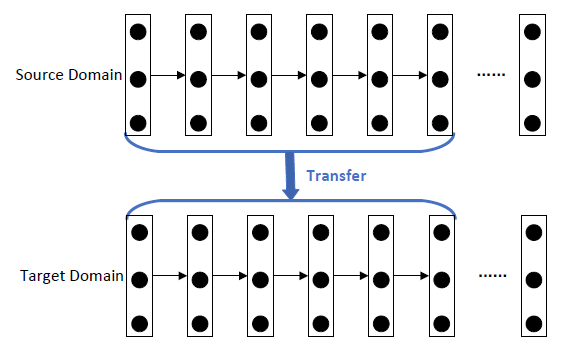
\includegraphics[width=0.9\linewidth]{transfer_learning_1.png}
    \caption{基于网络的迁移学习模型示意图}
    \label{fig:transfer_learning_1}
\end{figure}
\paragraph{}这篇文章\cite{6639081}也采用了相同的思路,实现了语音识别语言的功能。如图\ref{fig:transfer_learning_2}所示,作者将网络分成两个部分,前一部分是语言独立的特征提取器,最后一层是语言相关的分类器。神经网络的输入是不同语言的语音片段,经过共享的特征提取器,输出到最后的全连接层,从而可以达到识别语言种类的目的。文中指出,对于欧洲的四种语言,相比于使用单个语言训练的网络,单词的错误率下降了3\%-5\%。而对于英语和中文,相比于使用单个语言训练的网络,单词错误率下降了6\%-28\%。
\begin{figure}
    \centering
    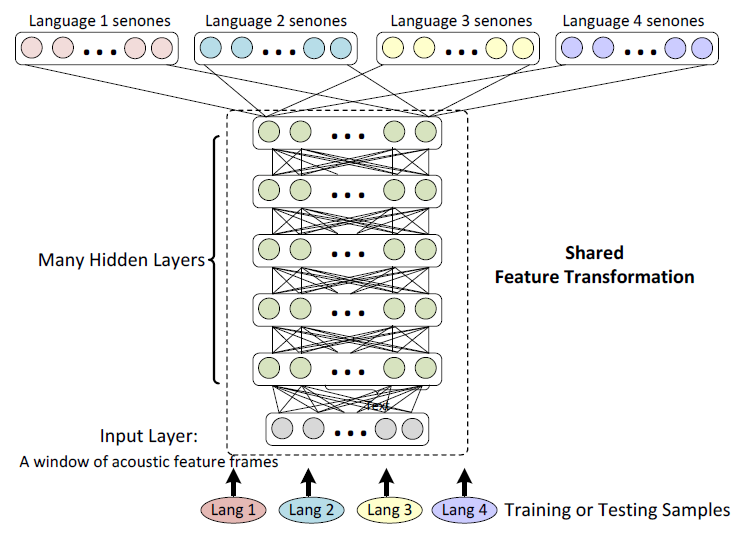
\includegraphics[width=0.9\linewidth]{transfer_learning_2.png}
    \caption{共享特征提取器的语言识别网络}
    \label{fig:transfer_learning_2}
\end{figure}
这篇文章\cite{Oquab_2014_CVPR}也讲到了共享特征提取器。如图\ref{fig:transfer_learning_5}所示,网络可以分成两个部分,一部分是卷积层,另一部分是全连接层。先将网络在一个训练集上训练,训练完成后,将卷积层和若干全连接层迁移到另外一个分类任务当中,替代网络中的卷积层和若干全连接层。为了更好地适应新的分类任务,作者新增了两层全连接层,然后使用新的训练集对网络进行训练,训练的同时冻结迁移过来的参数,只训练新增的全连接层的参数。训练至收敛后,网络同样取得了很好的效果。 
\begin{figure}
    \centering
    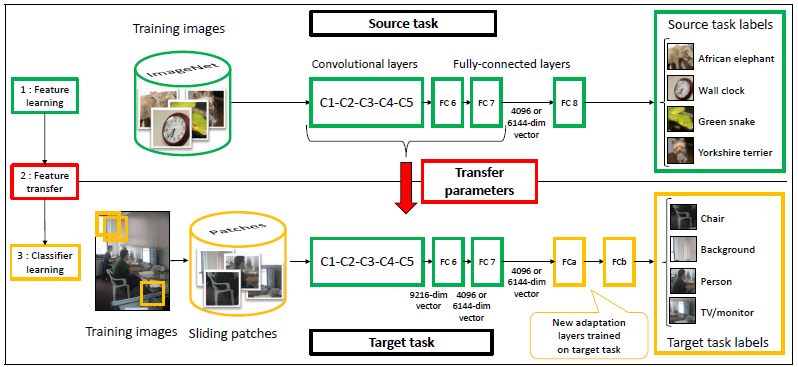
\includegraphics[width=0.9\linewidth]{transfer_learning_5.png}
    \caption{共享特征提取器的卷积神经网络}
    \label{fig:transfer_learning_5}
\end{figure}
这篇文章\cite{yosinski_2014_NIPS}对深度神经网络的特征可共享的特性进行了研究。如图\ref{fig:transfer_learning_3}所示,第一行代表用数据集1训练的网络,第二行代表用数据集2训练的网络。第三行代表将前三层参数冻结或者不冻结,并且将第二行前三层的参数迁移至第三行前三层参数。第四行代表前三层参数使用第一行训练好的前三层参数,之后的训练将这三层参数冻结或者不冻结进行训练。最终的结果如图\ref{fig:transfer_learning_4}所示,不冻结参数用不同数据集训练的网络得到了很好的泛化效果。从这个实验中可以看出,深度神经网络前若干层参数是可以共享的。
\begin{figure}
    \centering
    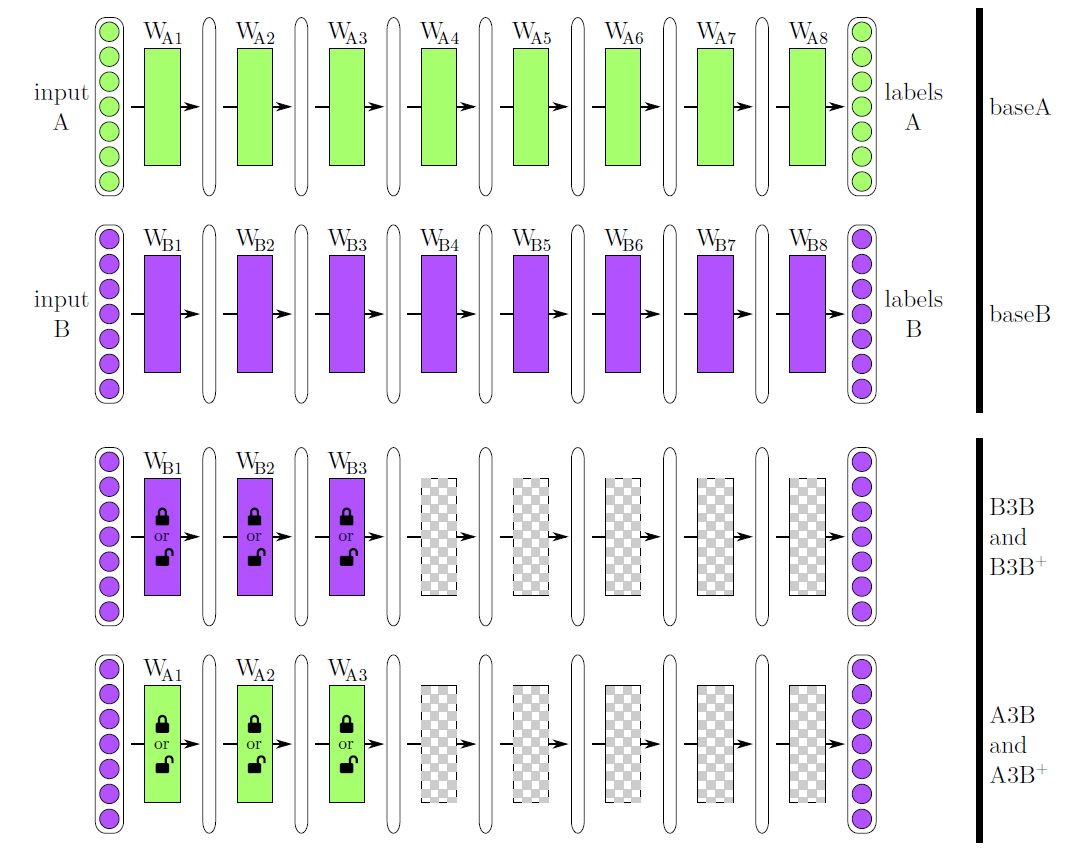
\includegraphics[width=0.9\linewidth]{transfer_learning_3.png}
    \caption{共享参数的深度神经网络训练示意图}
    \label{fig:transfer_learning_3}
\end{figure}
\begin{figure}
    \centering
    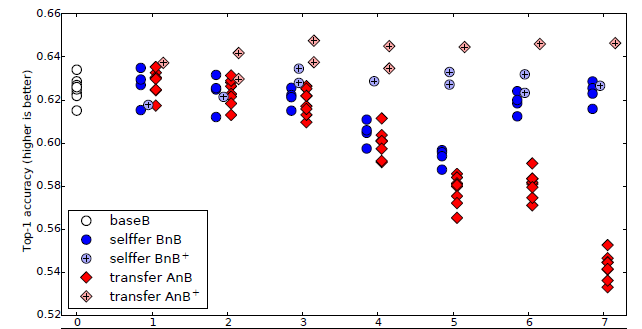
\includegraphics[width=0.9\linewidth]{transfer_learning_4.png}
    \caption{共享参数后实验结果}
    \label{fig:transfer_learning_4}
\end{figure}

\section{增量学习的研究}
增量学习\cite{PARISI201954}是指已经学习完成的机器学习模型继续学习新的数据的技术。增量学习遇到的挑战是灾难性遗忘,在已经学习完成的机器学习模型上只用新的数据集去训练会出现以前学习过的分类准确率出现下降的现象,就好像学习了新的知识将旧的知识忘记了。为了克服灾难性遗忘,这篇综述中提到增强学习大致可分为三种类型:基于正则化的方法,基于动态结构的方法以及基于补充学习系统(CLS)和记忆重放的方法。
增量学习的研究中,这篇文章\cite{8107520}是一篇具有代表性的文章。如图\ref{fig:incremental_learning_1}所示,图中展示了一个已经学习完成的网络在遇到新的学习任务时可能的学习方法。(a)中是原来已经学习好的模型,前半部分是卷积神经网络,后半部分是全连接层。当加入一个新的类别后,大概有三种可能的解决方法。一种是微调(fine-tuning),即在原来的网络上用新的训练数据直接训练。这样的方法会毫无疑问导致灾难性遗忘。第二种方法是联合训练(Joint Training),就是用新的训练数据和旧的训练数据同时训练原有的网络,这样带来的效果是比较好的,但是重新训练的成本是很大的。第三种方法是特征提取(Feature Extraction)的方法。和以前训练好的网络分享一部分参数,这部分参数不用来更新。然后用新的训练数据继续训练没有被冻结的参数。这样的方法可能的问题是新的训练数据的特有的特征无法被原有网络提取,因此最终的效果也不会很好。然而,遗忘和增量学习不同的是,遗忘学习是在原有的模型上做减法,所以不会涉及到新数据有特有特征的问题。
\begin{figure}
    \centering
    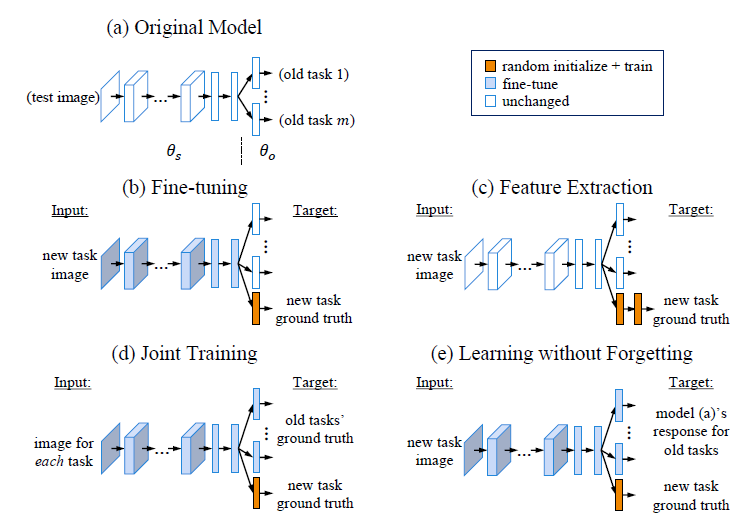
\includegraphics[width=0.9\linewidth]{incremental_learning_1.png}
    \caption{增量学习可能的方法分类}
    \label{fig:incremental_learning_1}
\end{figure}
这篇文章\cite{Sarwar_2020}通过共享网络层次,建立新网络分支来解决灾难性遗忘的问题。如图\ref{fig:incremental_learning_2}所示,原来的网络已经训练了50个类别,当有10个新的类别需要添加到网络中时,确定好共享网络,然后冻结共享网络和原来网络的网络参数,只用新的训练数据对新增加的网络进行训练。当需要做预测时,将两个网络的输出综合起来,判断应当输出的结果。这样的网络随着新增的类别不断增多而逐渐增大。但是我们可以看到共享网络参数的思想。
\begin{figure}
    \centering
    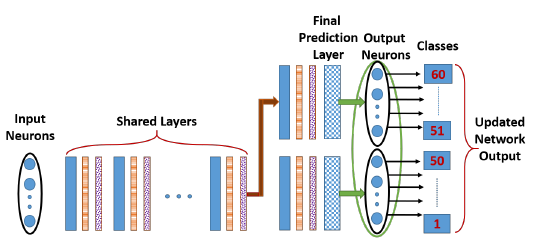
\includegraphics[width=0.9\linewidth]{incremental_learning_2.png}
    \caption{共享网络参数的增量学习}
    \label{fig:incremental_learning_2}
\end{figure}

\section{机器学习模型遗忘方法的研究}
\subsection{非卷积神经网络的遗忘方法}
这篇文章\cite{yinzhicao2015}最早引入了机器学习遗忘的研究,这篇文章使用统计查询学习的方法对基于贝叶斯方法的机器学习进行了遗忘算法的设计,并没有针对卷积神经网络设计遗忘算法。
这篇文章\cite{antonio2019}对于k-means机器学习的算法设计了遗忘某一类别的方法,可是仍然没有提及卷积神经网络的遗忘算法。
\subsection{基于分割网络的遗忘方法}
这篇文章\cite{2019arXiv191203817B}提出了一种可以用在神经网络上的遗忘方法。作者将训练数据集分成若干互不相交的部分,然后利用每个部分单独训练出一个神经网络模型,网络最终输出的结果将多个神经网络模型输出的结果综合起来,最终输出一个结果。遗忘的时候,只需要重新训练要遗忘的训练样例所在的神经网络,而无需重新训练所有模型,如图~\ref{fig:machine_unlearning}。这样的方式仍未摆脱重新训练的模式,而且训练如此多的神经网络也造成了参数的浪费。
\begin{figure}
    \centering
    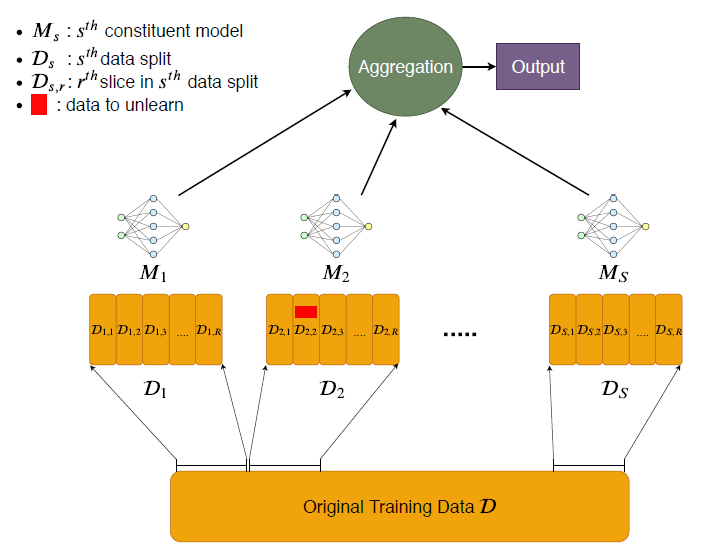
\includegraphics[width=0.9\linewidth]{machine_unlearning.png}
    \caption{将数据集分成若干互不相交集合分别训练}
    \label{fig:machine_unlearning}
\end{figure}
\begin{figure}
    \centering
    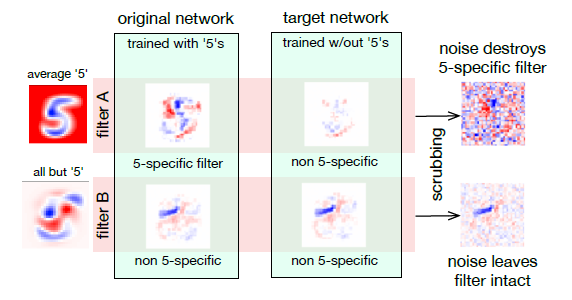
\includegraphics[width=0.9\linewidth]{eternal_sunshine.png}
    \caption{将数据集分成若干互不相交集合分别训练}
    \label{fig:eternal_sunshine}
\end{figure}
\subsection{基于增加噪音和正则化的遗忘方法}
这篇文章\cite{Golatkar_2020_CVPR}实现了一种通过在权重上增加噪音的方法来逐渐减少神经网络参数对遗忘数据的信息量,如图~\ref{fig:eternal_sunshine}。同时提出了一些衡量遗忘效果的指标,比如遗忘集的测试准确率,保留集(没有被遗忘的数据集)的测试准确率和测试集的测试准确率。还提出了模型信心的指标,就是对比目标神经网络与此文方法遗忘之后的网络针对遗忘集和保留集输出的交叉熵。这些指标在实际应用上具有参考价值,因此本文也参考了这些评价指标。这篇文章中还提到了一种信息论领域常用到的信息边界的衡量方法,就是计算两个网络模型参数的KL散度距离(Kullback-Leibler Divergence)。这种方法经常用于量化两个随机变量概率分布的相似性。然而,遗忘的目的并不只是简单地让网络的参数去接近目标网络就可以,因此这个衡量指标没有被本文所采用。这个方法虽然在遗忘的效果上达到了较为理想的状态,然而在没有遗忘的类别的准确率上面不是很理想。
这篇文章\cite{Golatkar_2021_CVPR}提出了一种混合训练模型,将训练集分为核心训练集和用户训练集。核心训练集表示学习后不会被遗忘的训练集,用户训练集代表学习后可能会被用户遗忘的训练集。文章中使用了两个神经网络用来训练。第一个网络只用核心训练集进行训练,第二个网络使用第一个网络的输出结果和用户训练集以及核心训练及一起进行训练。当用户申请遗忘数据时,系统会根据没有被遗忘的数据集还有训练好的第一个网络的权重,计算出一个权重变化差,记为$\Delta$w。第二个网络的权重减去这个$\Delta$w即可得到遗忘之后的权重。为了使遗忘的效果更加明显,减去$\Delta$w后再加上一定方差的噪声。文章使用的指标是遗忘集、保留集和测试集的准确率,重新学习时间,激活距离,还有伙伴推断攻击的成功率。激活距离定义为目标遗忘网络和这个方法遗忘后的网络对测试集输出差的第一范数值。伙伴推断攻击的目的是对于给定一个输入,通过一些方法和手段来判断这个输入是否被用于训练网络。其准确率被这篇文章用来当作评价遗忘效果的一个指标。本文借鉴了激活距离和伙伴推断攻击准确率这两个评价指标。


\section{本章小结}
